Il sistema si articola in due blockchain separate, la blockchain di firma e la blockchain di voto (da ora rispettivamente Signature chain o SC e Vote chain o VC). Le due chain sono isolate, per garantire la non collegabilità del voto al votante in fase di scrutinio.
Le due chain hanno scopi diversi: SC assicura che il voto avvenga in maniera controllata e abilita al voto il client, inoltre contiene le informazioni per dividere in raggruppamenti i votanti similmente a quanto avviene con le sezioni elettorali; VC raccoglie i voti e li registra per effettuare poi il conteggio, ma deve garantire l’anonimato del votante.

\section{Preparazione}
	Viene indetta una votazione. Si prevede che l'architettura sia già predisposta, in particolare devono essere noti ed affidabili, completi di chiavi pubbliche:
	\begin{itemize}
		\item L'elenco dei votanti;
		\item L'elenco dei peer;
		\item L'elenco degli indirizzi dei candidati per la Vote chain;
		\item L'elenco dei programmi client verificati.
	\end{itemize}
	\subsection{Inizializzazione della Signature chain}
		La SC viene predisposta con il chaincode che permette al client di interrogare la chain per conoscere le chiavi pubbliche dei votanti inseriti nello stesso raggruppamento, registrando contemporaneamente la propria firma. I dati sui raggruppamenti dei votanti sono inseriti nella SC. Questa dovrà essere accessibile solamente ai peer deputati al controllo della votazione, a causa della riservatezza delle informazioni sui raggruppamenti.
	\subsection{Inizializzazione della Vote chain}
		La VC contiene inizialmente delle transazioni che registrano l'associazione di ogni indirizzo numerico ad un nome intelleggibile del candidato corrispondente, i saldi dei voti dei candidati inizializzati a 0 e il chaincode necessario al client per incrementare di 1 il saldo del candidato scelto. Un altro chaincode utile è quello che permette ai peer di ricevere il conteggio finale e quindi l'esito della votazione, così come il chaincode che permette ad un servizio web di interrogare la blockchain e rendere pubblici i dati in essa contenuti per permettere al votante la verifica del voto espresso.

\section{Workflow di una votazione}
	\begin{figure}[ht]
		\centering
		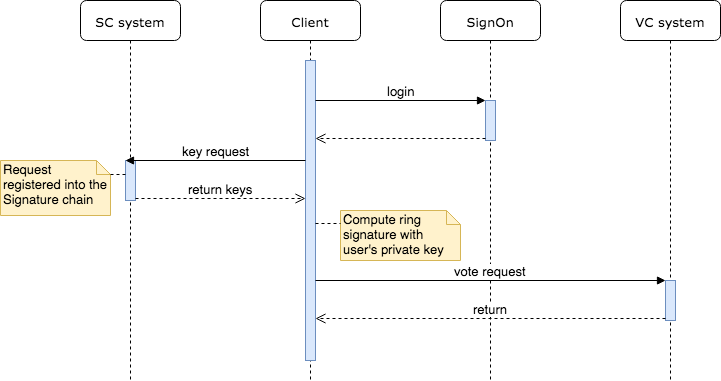
\includegraphics[width=\textwidth]{voting_workflow.png}
		\caption{Workflow della votazione}
		\label{fig:voting_workflow}
	\end{figure}
	Il diagramma in \hyperref[fig:voting_workflow]{figura \ref*{fig:voting_workflow}} illustra il workflow tipico di una votazione.
	\subsection{Signature chain: Firma del registro votanti}
		Il client autentica l'utente attraverso un \hyperref[subsec:personalita_voto]{sign-on affidabile}. I controlli di accesso possono essere rinforzati o meno da \hyperref[subsec:liberta_voto]{altri passaggi} affidati a sistemi di intelligenza artificiale o al controllo di un operatore. A utente autenticato, il client invoca il chaincode di query su SC ed ottiene l'elenco delle chiavi pubbliche del suo raggruppamento. Questa richiesta viene registrata in blockchain, per assicurarsi che lo stesso utente non possa ripetere la procedura di voto due volte.

	\subsection{Vote chain: In cabina elettorale}
		Il client si trova ora in possesso delle chiavi pubbliche della sua sezione. In locale permette al votante di esprimere la propria preferenza di voto e richiede la transazione corrispondente nella VC firmandola con la ring signature del proprio raggruppamento.
		La votazione è ora conclusa.

	\subsection{Scrutinio e verifica}
		Le operazioni di scrutinio e verifica possono ora essere completamente automatizzate, facendo riferimento ad una base di dati sicura e virtualmente inalterabile come la blockchain.